% 2015_jiangsu_q16_fig1: 直三棱柱 ABC-A1B1C1, D为AB1中点, E为B1C与BC1交点
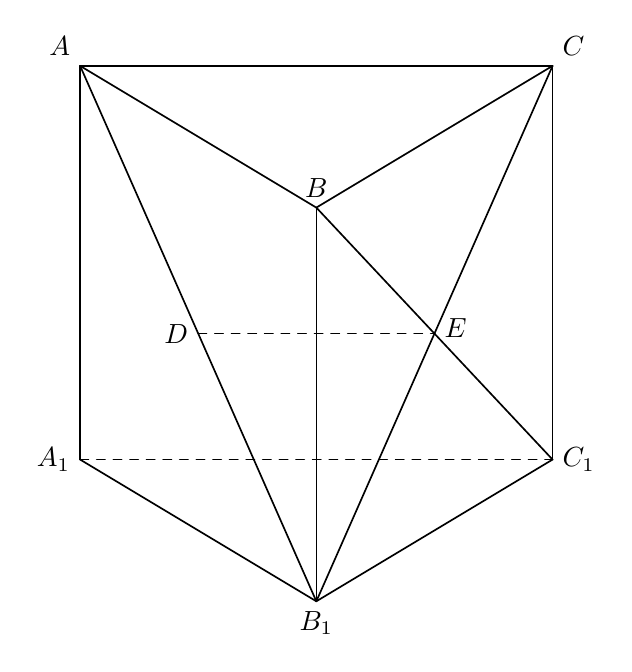
\begin{tikzpicture}[line width=0.6pt, line join=round, line cap=round, font=\normalsize]
\coordinate (A) at (0,6);
\coordinate (C) at (6,6);
\coordinate (B) at (3,4.2);
\coordinate (A1) at (0,1);
\coordinate (C1) at (6,1);
\coordinate (B1) at (3,-0.8);
\coordinate (E) at (4.5,2.6);
\coordinate (D) at (1.5,2.6);
% 顶面
\draw (A) -- (C);
\draw (A) -- (B);
\draw (C) -- (B);
% 侧棱
\draw (A) -- (A1);
\draw (C) -- (C1);
\draw (B) -- (B1);
% 底面
\draw[dashed] (A1) -- (C1);
\draw (A1) -- (B1);
\draw (C1) -- (B1);
% 内部连线
\draw (A) -- (B1);
\draw (C) -- (B1);
\draw (B) -- (C1);
\draw[dashed] (D) -- (E);
% 标签(避碰外置)
\node[above left] at (A) {$A$};
\node[above right] at (C) {$C$};
\node[above] at (B) {$B$};
\node[left] at (A1) {$A_{1}$};
\node[right] at (C1) {$C_{1}$};
\node[below] at (B1) {$B_{1}$};
\node[left] at (D) {$D$};
\node[right,xshift=0.00bp,yshift=2.00bp] at (E) {$E$};
\end{tikzpicture}
